% !TeX document-id = {6d425eb9-45a2-4fbe-9d0d-2f32c39ce2b6}
% !TeX TXS-program:compile = txs:///xelatex/[--shell-escape]
\documentclass[zihao=-4]{ctexart}

% 标题样式
\ctexset{
	% 二级标题样式
	section = {
		format = \raggedright \Large \heiti \bfseries
	}	
}

% 页面设置
\usepackage{geometry}
\geometry{top=2.0cm,bottom=2.0cm,left=2.2cm,right=2.2cm}
\pagestyle{empty}

% 图片
\usepackage{graphicx}

% 代码排版
%代码高亮,需要python,pygments支持和 -shell-escape
\usepackage{minted,xcolor}
\definecolor{LightGray}{rgb}{0.92,0.92,0.92}

% Matlab代码排版环境
\newminted[mcode]{matlab}{
	frame=none,
	framesep=2mm,
	baselinestretch=1.2,
	bgcolor=LightGray,
	fontsize=\footnotesize,
	linenos,
	showtabs=false,
	showspaces=false,
	breaklines
}
%% Pyhton 代码排版环境
\newminted[pycode]{python}{
	frame=none,
	framesep=2mm,
	baselinestretch=1.2,
	bgcolor=LightGray,
	fontsize=\footnotesize,
	linenos,
	showtabs=false,
	showspaces=false,
	breaklines
}

\usepackage{amsmath,amssymb}

\begin{document}
\begin{center}
{\zihao{2} \textbf{ 常用数学软件 \\ 第4次课堂练习}}
\\ \noindent
\begin{tabular}{cccccc}
	姓名:&   张三  &  学号:& 2022000000  &日期:  & \today 
\end{tabular}
\end{center}
	
\section*{一、练习目的}

\begin{enumerate}
	\item 掌握MATLAB的符号计算功能用于求解微积分问题 \vspace*{-1em}
	\item 掌握使用MATLAB解决高等代数问题。 \vspace*{-1em}
\end{enumerate}

\section*{二、练习内容}

\noindent
\textbf{练习1}: 使用MATLAB求解如下微积分问题,给出相应的程序和结果。

\begin{enumerate}
\item 使用符号计算功能验证如下公式的正确性。

\begin{itemize}
	\item 求极限
	$$
	\begin{gathered}
		\lim _{x \rightarrow 0} \frac{\sin x}{x} \\
		\lim _{n \rightarrow \infty}\left(1+\frac{1}{n}\right)^n
	\end{gathered}
	$$
	\item 下列函数的一阶和二阶偏导数
	$$
	\begin{gathered}
		f(x, y)=\sin x+x^3 e^y \\
		f(x, y)=e^x y+\sin \left(x^3\right) e^y
	\end{gathered}
	$$
	\item 计算如下的不定积分与定积分
	$$
	\begin{aligned}
		& \int_0^\pi \sin (2 x) d x \\
		& \int_0^{\infty} \frac{\sin x}{x} d x
	\end{aligned}
	$$
	\item 计算如下级数和
	$$
	\begin{aligned}
		& \sum_{k=1}^n k^2 \\
		& \sum_{k=1}^{\infty} \frac{1}{k^2}
	\end{aligned}
	$$
\end{itemize}

\item \textbf{Taylor展开式}:给出函数$\sin x^2$, 在点$x=1.0$处的3,5,7阶Taylor展开式,并绘制图像,观察taylor多项式逼近原函数的情况。给出原函数Taylor展开式的解析解;并将原函数和Taylor多项式绘制在同一张图中,观察逼近情况。(使用ezplot或fplot函数)
\end{enumerate}

\textbf{计算问题1的程序代码为}:
\begin{mcode}
 syms x y n k

% 1. 求极限
disp('1. 极限计算:');
limit1 = limit(sin(x)/x, x, 0)
limit2 = limit((1+1/n)^n, n, inf)

% 2. 偏导数计算
disp('2. 偏导数计算:');
f1 = sin(x) + x^3*exp(y);
df1_dx = diff(f1, x)
df1_dy = diff(f1, y)
d2f1_dx2 = diff(f1, x, 2)
d2f1_dy2 = diff(f1, y, 2)

f2 = exp(x)*y + sin(x^3)*exp(y);
df2_dx = diff(f2, x)
df2_dy = diff(f2, y)
d2f2_dx2 = diff(f2, x, 2)
d2f2_dy2 = diff(f2, y, 2)

% 3. 积分计算
disp('3. 积分计算:');
int1 = int(sin(2*x), x, 0, pi)
int2 = int(sin(x)/x, x, 0, inf)

% 4. 级数求和
disp('4. 级数求和:');
sum1 = symsum(k^2, k, 1, n)
sum2 = symsum(1/k^2, k, 1, inf)
\end{mcode}

\textbf{计算问题1的结果为}:
\begin{mcode}
1. 极限计算:
 limit1 =1
 limit2 =exp(1)
2. 偏导数计算:
 df1_dx =cos(x) + 3*x^2*exp(y)
 df1_dy =x^3*exp(y)
 d2f1_dx2 =6*x*exp(y) - sin(x)
 d2f1_dy2 =x^3*exp(y)
 df2_dx =y*exp(x) + 3*x^2*cos(x^3)*exp(y)
 df2_dy =exp(x) + sin(x^3)*exp(y)
 d2f2_dx2 =y*exp(x) - 9*x^4*sin(x^3)*exp(y) + 6*x*cos(x^3)*exp(y)
 d2f2_dy2 =sin(x^3)*exp(y)
3. 积分计算:
 int1 =0
 int2 =pi/2
4. 级数求和:
 sum1 =(n*(2*n + 1)*(n + 1))/6
 sum2 =pi^2/6
\end{mcode}


\textbf{计算问题2的程序代码为}:
\begin{mcode}
syms x
f = sin(x^2);
x0 = 1.0;

% 计算不同阶数的Taylor展开
t3 = taylor(f, x, 'ExpansionPoint', x0, 'Order', 3)
t5 = taylor(f, x, 'ExpansionPoint', x0, 'Order', 5)
t7 = taylor(f, x, 'ExpansionPoint', x0, 'Order', 7)

% 绘制图像
figure;
fplot(f, [0.5, 1.5], 'LineWidth', 2);
hold on;
fplot(t3, [0.5, 1.5], '--');
fplot(t5, [0.5, 1.5], ':');
fplot(t7, [0.5, 1.5], '-.');
legend('原函数 sin(x^2)', '3阶Taylor', '5阶Taylor', '7阶Taylor');
title('Taylor多项式逼近原函数');
grid on;
hold off;
\end{mcode}


\textbf{计算问题2的结果为}:
\begin{mcode}
t3 =sin(1) + (cos(1) - 2*sin(1))*(x - 1)^2 + 2*cos(1)*(x - 1)
t5 =sin(1) + (cos(1) - 2*sin(1))*(x - 1)^2 - (x - 1)^3*((4*cos(1))/3 + 2*sin(1)) - (x - 1)^4*(2*cos(1) - sin(1)/6) + 2*cos(1)*(x - 1)
t7 =sin(1) + (cos(1) - 2*sin(1))*(x - 1)^2 - (x - 1)^3*((4*cos(1))/3 + 2*sin(1)) - (x - 1)^4*(2*cos(1) - sin(1)/6) - (x - 1)^5*((11*cos(1))/15 - (4*sin(1))/3) + (x - 1)^6*(cos(1)/2 + (41*sin(1))/45) + 2*cos(1)*(x - 1)
\end{mcode}



\noindent
\textbf{练习2}:使用MATLAB求解如下代数问题, 给出计算分析,程序和结果.

\begin{enumerate}
\item 设向量组A为
	$$
	\alpha_1=\left[\begin{array}{c}
		1 \\
		-1 \\
		2 \\
		4
	\end{array}\right], \alpha_2=\left[\begin{array}{l}
		0 \\
		3 \\
		1 \\
		2
	\end{array}\right], \alpha_3=\left[\begin{array}{c}
		3 \\
		0 \\
		7 \\
		14
	\end{array}\right], \alpha_4=\left[\begin{array}{l}
		2 \\
		1 \\
		5 \\
		6
	\end{array}\right], \alpha_5=\left[\begin{array}{c}
		1 \\
		-1 \\
		2 \\
		0
	\end{array}\right]
	$$
	求向量组A的秩和一个极大无关组,并将其余向量用极大无关组线性表示。
	
\textbf{程序清单}:
	\begin{mcode}
A = [1 0 3 2 1;
    -1 3 0 1 -1;
    2 1 7 5 2;
    4 2 14 6 0];

% 求秩
rank_A = rank(A)

% 化为行最简形
rref_A = rref(A)

% 提取极大无关组(前rank_A列)
max_indep = A(:,1:rank_A)

% 将其他向量表示为极大无关组的线性组合
coefficients = rref_A(:,rank_A+1:end)
	\end{mcode}
\textbf{计算结果}:
\begin{mcode}
rank_A =3
rref_A =
	 1     0     3     0    -1
     0     1     1     0    -1
     0     0     0     1     1
     0     0     0     0     0
max_indep =
	 1     0     3
    -1     3     0
     2     1     7
     4     2    14
coefficients =
     0    -1
     0    -1
     1     1
     0     0
\end{mcode}	
\item 给出下述齐次方程组的基础解系和通解。
$$
\left\{\begin{array}{c}
	2 x_1+x_2+3 x_3+5 x_4-5 x_5=0 \\
	x_1+x_2+x_3+4 x_4-3 x_5=0 \\
	3 x_1+x_2+5 x_3+6 x_4-7 x_5=0
\end{array}\right.
$$

\textbf{程序清单}:
	\begin{mcode}
	syms x1 x2 x3 x4 x5
eq1 = 2*x1 + x2 + 3*x3 + 5*x4 - 5*x5 == 0;
eq2 = x1 + x2 + x3 + 4*x4 - 3*x5 == 0;
eq3 = 3*x1 + x2 + 5*x3 + 6*x4 - 7*x5 == 0;

[A,b] = equationsToMatrix([eq1,eq2,eq3],[x1,x2,x3,x4,x5]);
null_space = null(A)  % 基础解系
	\end{mcode}
\textbf{计算结果}:
\begin{mcode}
null_space =
[-2, -1, 2]
[ 1, -3, 1]
[ 1,  0, 0]
[ 0,  1, 0]
[ 0,  0, 1]
\end{mcode}
\item 求如下方阵的特征值和特征向量
$$
A=\left[\begin{array}{ccc}
	-2 & 1 & 1 \\
	0 & 2 & 0 \\
	-4 & 1 & 3
\end{array}\right]
$$

\textbf{程序清单}:
\begin{mcode}
	A = [-2 1 1;
     0 2 0;
     -4 1 3];

[V,D] = eig(A);
eigenvalues = diag(D)
eigenvectors = V
\end{mcode}
\textbf{计算结果}:
eigenvalues =
	-1
     2
     2
eigenvectors =
   -0.7071   -0.2425    0.3015
         0         0    0.9045
   -0.7071   -0.9701    0.3015


\item 如图~\ref{fig:fig1}是某区的城市交通图,假设所有道路都是单行道,且道上不能停车,通行方向用箭头已经表明,数字代表某时段该路段的车辆数.假设进入每个交叉点的车辆数等于离开该交叉点的车辆数.请求出该时段没有标出的各路线的车辆数. 

\begin{figure}[H]
	\centering
	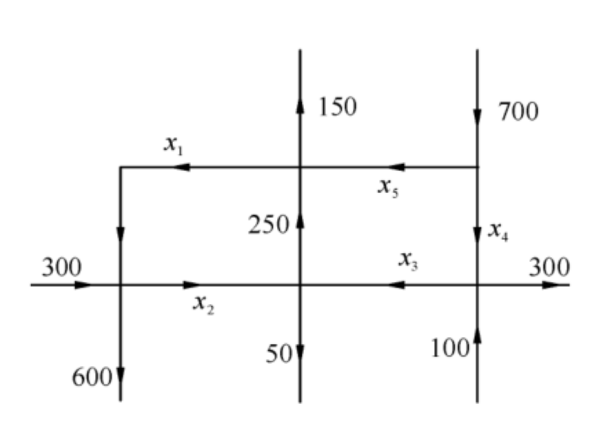
\includegraphics[width=0.7\linewidth]{fig1}
	\caption{某区域交通流量图}
	\label{fig:fig1}
\end{figure}


\textbf{程序清单}:
\begin{mcode}
	syms x1 x3 x4 x5

% 定义方程组
eq1 = x1 + 300 == 250 + 100;        % 左上交叉点
eq2 = 250 + 50 == x5 + 600;         % 右上交叉点
eq3 = 100 + x3 == x1 + 700;         % 左下交叉点
eq4 = x5 + 700 == x4 + 600;         % 右下交叉点

% 求解方程组
sol = solve([eq1, eq2, eq3, eq4], [x1, x3, x4, x5]);

% 显示结果
disp('解为:');
disp(['x1 = ', num2str(double(sol.x1))]);
disp(['x3 = ', num2str(double(sol.x3))]);
disp(['x4 = ', num2str(double(sol.x4))]);
disp(['x5 = ', num2str(double(sol.x5))]);
\end{mcode}
\textbf{计算结果}:
\begin{mcode}
解为:
x1 = 50
x3 = 650
x4 = -200
x5 = -300
\end{mcode}
\end{enumerate}


\end{document}